%++++++++++++++++++++++++++++++++++++++++
% Don't modify this section unless you know what you're doing!
%\documentclass[letterpaper,12pt]{article}
\documentclass[a4paper]{article}
\usepackage{tabularx} % extra features for tabular environment
\usepackage{amsmath}  % improve math presentation
\usepackage{graphicx} % takes care of graphic including machinery
%\usepackage[margin=1in,letterpaper]{geometry} % decreases margins
\usepackage{cite} % takes care of citations
%\usepackage[final]{hyperref} % adds hyper links inside the generated pdf file
%\hypersetup{
%	colorlinks=true,       % false: boxed links; true: colored links
%	linkcolor=blue,        % color of internal links
%	citecolor=blue,        % color of links to bibliography
%	filecolor=magenta,     % color of file links
%	urlcolor=blue         
%}
%++++++++++++++++++++++++++++++++++++++++
\usepackage{indentfirst}
\usepackage{tensor}
\usepackage{amssymb}
\allowdisplaybreaks
\usepackage{bm}
\newcommand{\at}[2][]{#1|_{#2}}
\newcommand\numberthis{\addtocounter{equation}{1}\tag{\theequation}}
\newcommand\norm[1]{\left\lVert#1\right\rVert}

\begin{document}

\title{CoM Estimation on the HRP4 Humanoid\\(draft)}
\author{Michele Cipriano, Godwin Joey, Lorenzo Vianello\\Supervised by Nicola Scianca}
\date{\today}
\maketitle

%\begin{abstract}
%In this experiment we studied a very important physical effect by measuring the
%dependence of a quantity $V$ of the quantity $X$ for two different sample
%temperatures.  Our experimental measurements confirmed the quadratic dependence
%$V = kX^2$ predicted by Someone's first law. The value of the %mystery parameter
%$k = 15.4\pm 0.5$~s was extracted from the fit. This value is
%not consistent with the theoretically predicted $k_{theory}=17.34$~s. We attribute this
%discrepancy to low efficiency of our $V$-detector.
%\end{abstract}


\section{Introduction}

General overview of the project, what has been implemented,
etc\cite{DBLP:journals/arobots/OrioloPRV16}.


\section{Torso Pose Estimation}
Brief introduction to the section.

\subsection{Kinematic Model}
Let $\bm{x} = (\bm{p}_t^T, \bm{o}_t^T)^T$ be the pose of the torso frame $\mathcal{F}_t$
with respect to the world frame $\mathcal{F}_w$. We want to
develop a filter that estimates the state of $\bm{x}$ while
it moves around the environment. Let $\mathcal{F}_s$ be the
support foot frame with respect to the world frame and let
$\bm{o}_s$ be the its orientation.
Let $\bm{J}(\bm{q}_s, \bm{o}_s)$ the Jacobian
matrix of the kinematic map from the support frame 
$\mathcal{F}_s$ to the torso frame $\mathcal{F}_t$.
Let's use the following kinematic model to describe the
evolution of the state $\bm{x}$ through time:
\begin{equation}
    \bm{\dot{x}} = \bm{J}(\bm{q}_s, \bm{o}_s) \bm{\dot{q}}_s
    \label{eq:hrp4-kinematic-model}
\end{equation}

\noindent with $\bm{\dot{q}}_s$ velocities of the support joints
acting as control inputs. Note that the Jacobian
$\bm{J}(\bm{q}_{s}, \bm{o}_s)$ does not depend on the
position of $\mathcal{F}_s$:
\begin{align*}
    \bm{f}(\bm{q}_s, \bm{o}_s) &= \bm{\varOmega} \left(
        \begin{bmatrix}
            \bm{R}_z(\bm{o}_s) & \bm{0} \\
            \bm{0}^T & 1 
        \end{bmatrix}
        \bm{\varOmega}^{-1}\left(
        \begin{bmatrix}
             \tensor[^s]{\bm{p}}{_t} \\
             \tensor[^s]{\bm{o}}{_t}
        \end{bmatrix}
        \right)
        \right) \\
        &= \bm{\varOmega} \left(
        \begin{bmatrix}
            \bm{R}_z(\bm{o}_s) & \bm{0} \\
            \bm{0}^T & 1 
        \end{bmatrix}
         \begin{bmatrix}
            \tensor[^s]{\bm{R}}{_t}(\tensor[^s]{\bm{o}}{_t}) & \tensor[^s]{\bm{p}}{_t} \\
            \bm{0}^T & 1 
        \end{bmatrix}
        \right) \\
        &= \bm{\varOmega} \left(
        \begin{bmatrix}
            \bm{R}_z(\bm{o}_s) \tensor[^s]{\bm{R}}{_t}(\tensor[^s]{\bm{o}}{_t}) & \bm{R}_z(o_s) \tensor[^s]{\bm{p}}{_t}  \\
            \bm{0}^T & 1 
        \end{bmatrix}
        \right) \\
        &= \bm{\varOmega} \left(
        \begin{bmatrix}
            \bm{R}_z(\bm{o}_s) \bm{R}_z(\tensor[^s]{\bm{o}}{_{t,z}}) \bm{R}_y(\tensor[^s]{\bm{o}}{_{t,y}}) \bm{R}_x(\tensor[^s]{\bm{o}}{_{t,x}}) & \bm{R}_z(o_s) \tensor[^s]{\bm{p}}{_t}  \\
            \bm{0}^T & 1 
        \end{bmatrix}
        \right) \\
        &= \bm{\varOmega} \left(
        \begin{bmatrix}
            \bm{R}_z(\bm{o}_s + \tensor[^s]{\bm{o}}{_{t,z}}) \bm{R}_y(\tensor[^s]{\bm{o}}{_{t,y}}) \bm{R}_x(\tensor[^s]{\bm{o}}{_{t,x}}) & \bm{R}_z(\bm{o}_s) \tensor[^s]{\bm{p}}{_t}  \\
            \bm{0}^T & 1 
        \end{bmatrix}
        \right) \\
        &=
        \begin{pmatrix}
            \bm{R}_z(\bm{o}_s) \tensor[^s]{\bm{p}}{_t} \\
            \tensor[^s]{\bm{o}}{_{t,x}} \\
            \tensor[^s]{\bm{o}}{_{t,y}} \\
            \bm{o}_s + \tensor[^s]{\bm{o}}{_{t,z}}
        \end{pmatrix} \\
        &=
        \begin{bmatrix}
            \bm{R}_z(\bm{o}_s) & \bm{O} \\
            \bm{O} & \bm{I}
        \end{bmatrix}
        \begin{pmatrix}
            \tensor[^s]{\bm{p}}{_t} \\
            \tensor[^s]{\bm{o}}{_t}
        \end{pmatrix}
        +
        \begin{pmatrix}
            \bm{0}_{5} \\
            \bm{o}_s
        \end{pmatrix} \\
        &=
        \begin{bmatrix}
            \bm{R}_z(\bm{o}_s) & \bm{O} \\
            \bm{O} & \bm{I}
        \end{bmatrix}
        \bm{f}(\bm{q}_s)
        +
        \begin{pmatrix}
            \bm{0}_{5} \\
            \bm{o}_s
        \end{pmatrix} \numberthis \\
    \bm{J}(\bm{q}_s, \bm{o}_s) &= \frac{\partial \bm{f}(\bm{q}_s, \bm{o}_s)}{\partial \bm{q}_s} \\
    &= 
    \begin{bmatrix}
            \bm{R}_z(\bm{o}_s) & \bm{O} \\
            \bm{O} & \bm{I}
    \end{bmatrix}
    \frac{\partial \bm{f}(\bm{q}_s)}{\partial \bm{q}_s} \\
    &=
    \begin{bmatrix}
            \bm{R}_z(\bm{o}_s) & \bm{O} \\
            \bm{O} & \bm{I}
    \end{bmatrix}
    \bm{J}(\bm{q}_s) \numberthis
\end{align*}

\noindent which definition is important for development purposes.
In fact, $\bm{J}(\bm{q}_s)$ is easily accessible thanks to the
C++ implementation of the HRP4 kinematics. Note that, unless
specified otherwise, $\bm{I} \in \mathbb{R}^{3 \times 3}$
represents the identity matrix,
$\bm{O} \in \mathbb{R}^{3 \times 3}$
represents the zero matrix, while $\bm{0} \in \mathbb{R}^{3}$ 
represents the zero vector. $\bm{\varOmega}$ is a function that
returns a minimal representation of a transform function.
In the C++ library \texttt{Eigen}, $\bm{\varOmega}$ is
implemented
with \texttt{t2v}, while $\bm{\varOmega}^{-1}$ is implemented
with \texttt{v2t}.

The robot is equipped with a RGBD camera and an IMU, used
to measure the pose of the torso frame:
\begin{equation}
    \bm{y} = \bm{h}(\bm{x}, \bm{q}_n) =
        \begin{pmatrix}
            \bm{p}_t \\
            \bm{o}_t
        \end{pmatrix}
    \label{eq:ekf-observation-function}
\end{equation}

In particular, the position $\bm{p}_t$ is computed by doing
trilateration exploiting known position of the landmarks, while
the orientation $\bm{o}_t$ is computed by simply integrating
the data obtained from the IMU. Details are explained in
subsections \ref{subsec:gyro-integration} and
\ref{subsec:trilateration}. [TODO: ADD COMMENT ABOUT
NOTATION OF $q_s$ AND $q_n$ WHICH IS CONSISTENT WITH
THE PAPER BUT NOT ACTUALLY USED IN THE IMPLEMENTATION].

\subsection{Extended Kalman Filter}
It is now possible to define a discrete-time stochastic system
using equations (\ref{eq:hrp4-kinematic-model},
\ref{eq:ekf-observation-function}), with $T$ sampling
interval of the filter and $k$ current timestep:
\begin{align}
    \bm{x}_{k+1} &= \bm{x}_k + T \bm{J}(\bm{q}_{s,k}, \bm{o}_s) \bm{\dot{q}}_{s,k} + \bm{v}_k \\
    \bm{y}_k &= \bm{h}(\bm{x}_k, \bm{q}_{n,k}) + \bm{w}_k
\end{align}

\noindent with $\bm{v}_k \sim \bm{\mathcal{N}}(\bm{0}, \bm{V}_k)$ and $\bm{w}_k \sim \bm{\mathcal{N}}(\bm{0}, \bm{W}_k)$ zero-mean
white Gaussian noises and
$\bm{V}_k \in \mathbb{R}^{6 \times 6}$,
$\bm{W}_k \in \mathbb{R}^{6 \times 6}$ their respective
covariance matrices.

%%% EKF Prediction.

At each timestep, a prediction $\bm{\hat{x}}_{k+1|k}$ is
generated using the current estimate $\bm{\hat{x}}_{k}$:
\begin{equation}
    \bm{\hat{x}}_{k+1|k} = \bm{\hat{x}}_k + \bm{J}(\bm{q}_{s,k}, \bm{o}_s) \Delta \bm{q}_{s,k},
    \quad \Delta \bm{q}_{s,k} = \bm{q}_{s,k+1} - \bm{q}_{s,k}
\end{equation}

\noindent with $\Delta \bm{q}_{s,k} \approx T \bm{\dot{q}}_{s,k}$
obtained using encoder readings. The covariance prediction
matrix is updated accordingly:
\begin{equation}
    \bm{P}_{k+1|k} = \bm{P}_{k} + \bm{V}_{k}
\end{equation}

In the same way as before, the predicted output
associated to $\bm{\hat{x}}_{k+1|k}$ is computed as well:
\begin{equation}
    \bm{\hat{y}}_{k+1|k} = \bm{h}(\bm{\hat{x}}_{k+1|k}, \bm{q}_{n, k+1})
\end{equation}

%%% EKF Correction.
To correct the predicted state we need to compute the
innovation using the measurements and the predicted
output computed in the previous step:
\begin{equation}
    \bm{\nu}_{k+1} = \bm{y}_{k+1} - \bm{\hat{y}}_{k+1|k}
\end{equation}

It is, hence, possible to determine the corrected state
estimate by computing:
\begin{equation}
    \bm{\hat{x}}_{k+1} = \bm{\hat{x}}_{k+1|k} + \bm{G}_{k+1} \bm{\nu}_{k+1}
\end{equation}

\noindent with $\bm{G}_{k+1}$ Kalman gain matrix, defined as
\begin{align}
    \bm{G}_{k+1} &= \bm{P}_{k+1|k} \bm{H}_{k+1}^T \left( \bm{H}_{k+1} \bm{P}_{k+1|k} \bm{H}_{k+1}^T + \bm{W}_{k+1} \right)^{-1} \\
        &= \bm{P}_{k+1|k} (\bm{P}_{k+1|k} + \bm{W}_{k+1})^{-1}
\end{align}

\noindent since the partial derivative of the observation
function with respect to the state is the identity matrix:
\begin{align}
    \bm{H}_{k+1} = \frac{\partial \bm{h}}{\partial \bm{x}} \at[\bigg]{\bm{x}=\bm{\hat{x}}_{k+1|k}} 
        = I
\end{align}

The corrected covariance matrix is updated as well:
\begin{align}
    \bm{P}_{k+1} &= \bm{P}_{k+1|k} - \bm{G}_{k+1} \bm{H}_{k+1} \bm{P}_{k+1|k} \\
        &= \bm{P}_{k+1|k} - \bm{G}_{k+1} \bm{P}_{k+1|k}
\end{align}

Note that, in our implementation, we defined the covariance
matrices $\bm{V}$ and $\bm{W}$ as [TODO]:
\begin{align}
    \bm{V} &= \text{diag}\{\cdot\} \\
    \bm{W} &= \text{diag}\{\cdot\}
\end{align}

\subsection{Gyroscope Integration}
\label{subsec:gyro-integration}
Gyroscope integration (Euler).
\begin{equation}
    \bm{o}_{t,k+1} = \bm{o}_{t,k} + T \bm{\dot{o}}_{t,k}
\end{equation}

Gyroscope integration (Trapezoidal).
\begin{equation}
    \bm{o}_{t,k+1} = \bm{o}_{t,k} + T \frac{\bm{\dot{o}}_{t,k} + \bm{\dot{o}}_{t,k-1}}{2}
\end{equation}

Note that the implementation of the gyroscope returns, at each
timestep $k$, the angular velocity
$\tensor[^t]{\bm{\dot{o}}}{_{t,k}}$ expressed in the current
reference frame of the torso, hence, it must be transformed to
the reference frame of the world in order be able to perform the
integration:
\begin{equation}
    \bm{\dot{o}}_{t,k} = [\tensor[]{\bm{T}}{_{RPY}}(\bm{\hat{x}}_{k+1|k})]^{-1} \tensor[^t]{\bm{\dot{o}}}{_{t,k}}
\end{equation}

\noindent with:
\begin{equation}
    \tensor[]{\bm{T}}{_{RPY}}(\bm{\hat{x}}_{k+1|k}) =
    \begin{pmatrix}
        cos(\beta) cos(\gamma) & -sin(\gamma) & 0 \\
        cos(\beta) sin(\gamma) &  cos(\gamma) & 0 \\
        -sin(\beta) & 0 & 1
    \end{pmatrix}
\end{equation}

\noindent where $\beta$ and $\gamma$ are, respectively,
the pitch and the yaw angles of $\bm{\hat{x}}_{k+1|k}$.
%\noindent where $\tensor[^w]{\bm{R}}{_t}(\bm{\hat{x}}_{k+1|k})$ represents
%the rotation matrix
%from the reference frame of the torso to the reference frame
%of the world (roll-pitch-yaw angles determined by the %estimate
%$\bm{\hat{x}}_{k+1|k}$).%, while $\tensor[^t]{\bm{\dot{o}}}{_{t,k}}$
%represents the angular velocity of the torso expressed in the
%reference frame of the torso at time $k$.

\subsection{Trilateration}

[TODO: DESCRIBE PROBLEMS WITH DOUBLE INTEGRATION OF THE
ACCELEROMETER].

\label{subsec:trilateration}
Let's now discuss how
trilateration\cite{trilateration-hereman-1995} can be used with
a RGBD camera in order to obtain the position of the torso
$\bm{p}_t$. We will find the position $\bm{p}_h$ of the camera
in order to obtain the position of the torso.

First, it's important to have landmarks that can be
easily recognizable. To achieve this, we have added to the scene
$n=6$ spheres of different colors. The camera of the robot is
pointing towards the
sky in order to simplify the recognition of the spheres
themselves avoiding the colors of the terrain.
Moreover, the specular, the emissive and the auxiliary
components of the spheres are the same as their ambient component
in order to avoid shades. This allows to have pixels of the same
color when seeing a sphere. It is, hence, possible to obtain
the pixel coordinates $(p_x, p_y)^T$ of each sphere in the image
of the camera by computing the centroid (a simple weighted mean
in our implementation) of the sphere itself.

Let $w$ and $h$ be the width and the
height of the images coming from the RGB camera. Let $\lambda$ be
the focal length (length to the nearest clipping
plane), $\lambda_f$ be length to the furthest clipping plane and
$\phi$ be the perspective angle of the camera. It is possible
to obtain the position (expressed with respect to
the reference frame of the camera) of each sphere with centroid
at coordinates $(p_x, p_y)^T$ by simply considering the proportion
between the ratio of the pixel coordinates (translated so
that the origin is at $(0, 0)^T$) and half the size of the
image (in particular width when computing the $x$ component,
height when computing the $y$ component), and the ratio between
the coordinates of the sphere (in camera frame) and the distance
between the considered point with the axes $x$ and $y$ of the
camera frame. This results in a simple computation:
\begin{align}
    \tensor[^{cam}]{x}{} = \frac{2 p_x - w}{w} \tensor[^{cam}]{z}{} \cdot tan\left(\frac{\phi}{2}\right) \\
    \tensor[^{cam}]{y}{} = \frac{2 p_y - h}{h} \tensor[^{cam}]{z}{} \cdot tan\left(\frac{\phi}{2}\right) 
\end{align}

\noindent with $(\tensor[^{cam}]{x}{}, \tensor[^{cam}]{y}{},
\tensor[^{cam}]{z}{})^T$ coordinates of the considered point
in the camera frame. Note that $\tensor[^{cam}]{z}{}$ can be
computed by
considering the distance from the clipping planes and the
depth $p_z$ of the object at position $(p_x, p_y)^T$, which can
be obtained by using the depth sensor of the RGBD camera:
\begin{equation}
    \tensor[^{cam}]{z}{} = (\lambda_f - \lambda) \cdot p_z + \lambda
\end{equation}

Moreover, note that the depth sensor returns a value between $0$ and $1$.
In particular, it returns $0$ if a point is exactly
on the nearest clipping plane, $1$ if a point is exactly on the
furthest clipping plane.

Given that each sphere has radius $\bar{r}$, it is possible to
obtain the distance from the camera to each sphere $i$ by computing:
\begin{equation}
    r_i =
    \norm{
        \begin{pmatrix}
            \tensor[^{cam}]{x}{_i} \\
            \tensor[^{cam}]{y}{_i} \\
            \tensor[^{cam}]{z}{_i}
        \end{pmatrix}
    }^2 + \bar{r} \quad (i = 1, 2, \dots, n)
\end{equation}

\noindent where the subscript $i$ specifies the index of the
sphere. Note that adding $\bar{r}$ to the norm is an
approximation of the real distance since the centroid could
not be along the line passing through the position of the
camera and the center of the sphere (e.g. when a sphere is
only partially visible because occluded by another sphere or
clipped).

[TODO: SAY WHICH ARE THE VALUES USED IN THE IMPLEMENTATION].

Since the position of the spheres $(x_i, y_i, z_i)^T$ is known
and it is possible
to associate the distance $r_i$ to each sphere because of the
unique color, the problem of finding the position of the 
camera $\bm{p}_h$ is reduced to solving the following system of equations:
\begin{equation}
    (p_{h,x} - x_i)^2 + (p_{h,y} - y_i)^2 + (p_{h,z} - z_i)^2 = r_i^2 \quad (i = 1, 2, \dots, n)
\end{equation}

\noindent which can we rewritten as a linear system of equations
$\bm{Ax} = \bm{b}$, where:
\begin{equation}
    \bm{A} = \begin{pmatrix}
            x_2 - x_1 & y_2 - y_1 & z_2 - z_1 \\
            x_3 - x_1 & y_3 - y_1 & z_3 - z_1 \\
            \vdots & \vdots & \vdots \\
            x_n - x_1 & y_n - y_1 & z_n - z_1
        \end{pmatrix}, \quad
    \bm{x} =
        %\begin{pmatrix}
        %    x - x_1 \\
        %    y - y_1 \\
        %    z - z_1
        %\end{pmatrix}, \quad 
        \bm{p}_h - 
        \begin{pmatrix}
            x_1 \\
            y_1 \\
            z_1
        \end{pmatrix}, \quad 
    \bm{b} = \begin{pmatrix}
            b_{21} \\
            b_{31} \\
            \vdots \\
            b_{n1}
        \end{pmatrix}
\end{equation}

\noindent where each element of the vector $b$ is defined as:
\begin{equation}
    b_{k1} = \frac{1}{2}\left[ r_1^2 + r_k^2 + (x_k - x_1)^2 + (y_k - y_1)^2 + (z_k - z_1)^2 \right] \quad (k = 2, 3, \dots, n)
\end{equation}

\noindent hence, the position of the camera can be determined by:
\begin{equation}
    %\begin{pmatrix}
    %    x \\
    %    y \\
    %    z 
    %\end{pmatrix}
    \bm{p}_h
        =
    \bm{x} + 
    \begin{pmatrix}
        x_1 \\
        y_1 \\
        z_1 
    \end{pmatrix}
\end{equation}

[TODO: DESCRIBE THE USE OF THE
PSEUDOINVERSE (MINIMIZATION PROBLEM), THE MINIMUM NUMBER OF POINT (4) NEEDED TO DO TRILATERATION]

At this point, the position of the torso can be obtained by
a simple transformation:
\begin{equation}
    \bm{p}_t = \bm{p}_h - \tensor[^w]{\bm{R}}{_t}(\bm{\hat{x}}_{k+1|k}) (\tensor[^t]{\bm{p}}{_h} - \tensor[^t]{\bm{p}}{_t})
\end{equation}

\noindent with $\tensor[^t]{\bm{p}}{_h} - \tensor[^t]{\bm{p}}{_t}$
constant and known
since the camera has been defined as child of the torso in
the hierarchical model of the robot in order to simplify the
computation of the direct kinematics.

\section{MPC Loop Closure}
[TODO: DESCRIPTION OF THE MPC AS DONE ABOVE WITH EKF].

\section{Experiments}
[TODO: DIVIDE THIS SECTION IN SUBSECTIONS].

Figures \ref{fig:comp-ground-truth-estimated-torso} and
\ref{fig:diff_ground_truth_estimated_torso} for the
torso pose estimation (\texttt{simulationType = 1}) [TODO:
ADD DESCRIPTION].

[TODO: ADD FIGURES OF THE ROBOT FOLLOWING A STRAIGHT LINE].

[TODO: DOUBLE CHECK THAT THE TORSO POSE ESTIMATION IS
ACTUALLY USEFUL TO FOLLOW THE RIGHT TRAJECTORY].

Figures \ref{fig:comp_estimated_torso_com} and \ref{fig:diff_estimated_torso_com} for the torso position
estimate and the CoM. Is there actually a way to use this
for the MPC loop closure? Note, moreover, that the
implementation of the MPC is using the position of the
CoM w.r.t. the reference frame of the support foot, which
is independent from the pose of the torso.

\begin{figure}
    \centering
    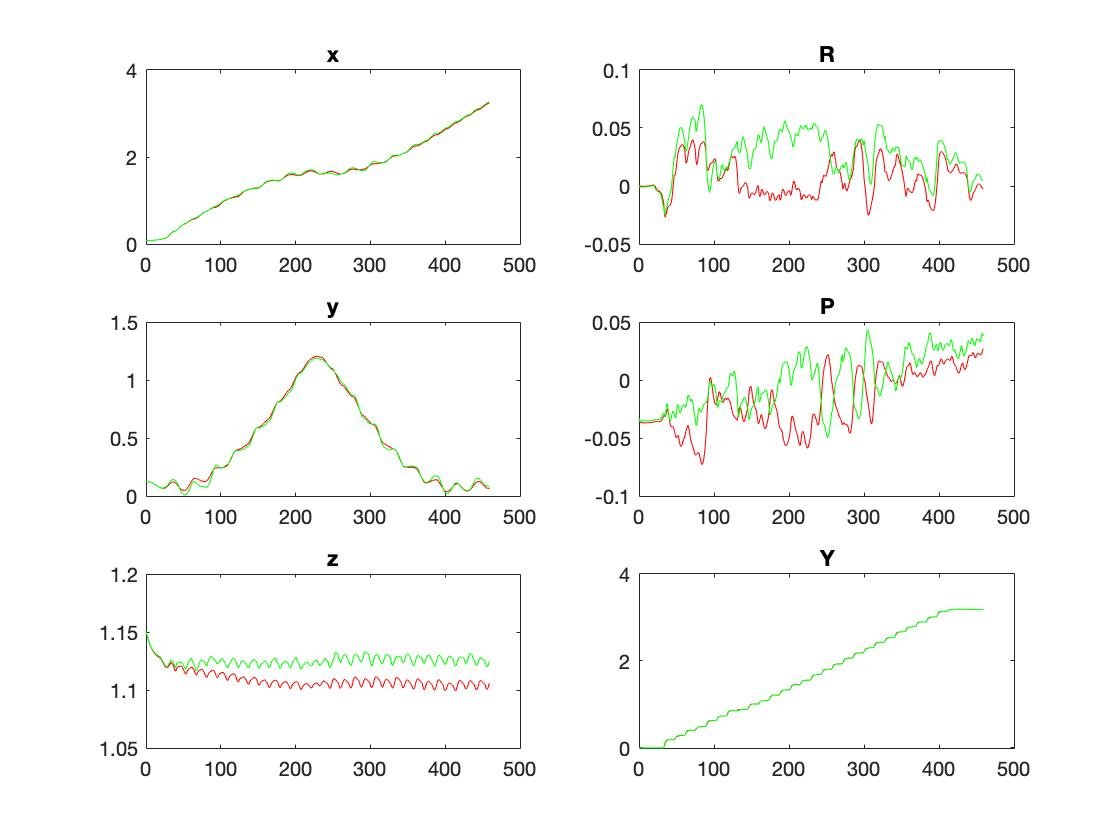
\includegraphics[width=\textwidth]{images/comp_ground_truth_estimated_torso.jpg}
    \caption{Comparison of the pose of the torso estimated
        with the EKF (in red) with respect to the ground
        truth (in green). $x$, $y$, $z$ stands for the position
        of the torso expressed in the reference frame of the
        world. $R$, $P$, $Y$ stands for the rotations roll,
        pitch, yaw around the respective axes of the
        reference frame of the world.}
    \label{fig:comp-ground-truth-estimated-torso}
\end{figure}

\begin{figure}
    \centering
    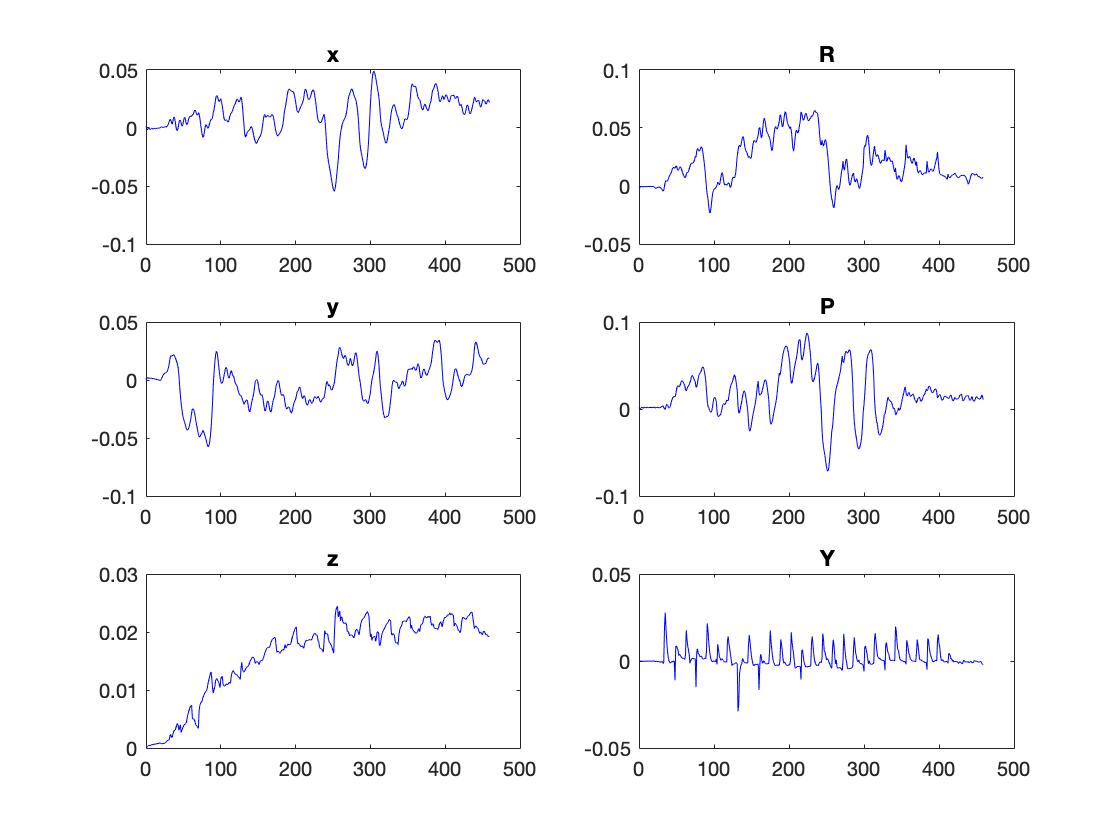
\includegraphics[width=\textwidth]{images/diff_ground_truth_estimated_torso.jpg}
    \caption{Difference of the pose of the torso estimated
        with the EKF (in red) with respect to the ground
        truth (in green). $x$, $y$, $z$ stands for the position
        of the torso expressed in the reference frame of the
        world. $R$, $P$, $Y$ stands for the rotations roll,
        pitch, yaw around the respective axes of the
        reference frame of the world.}
    \label{fig:diff_ground_truth_estimated_torso}
\end{figure}

\begin{figure}
    \centering
    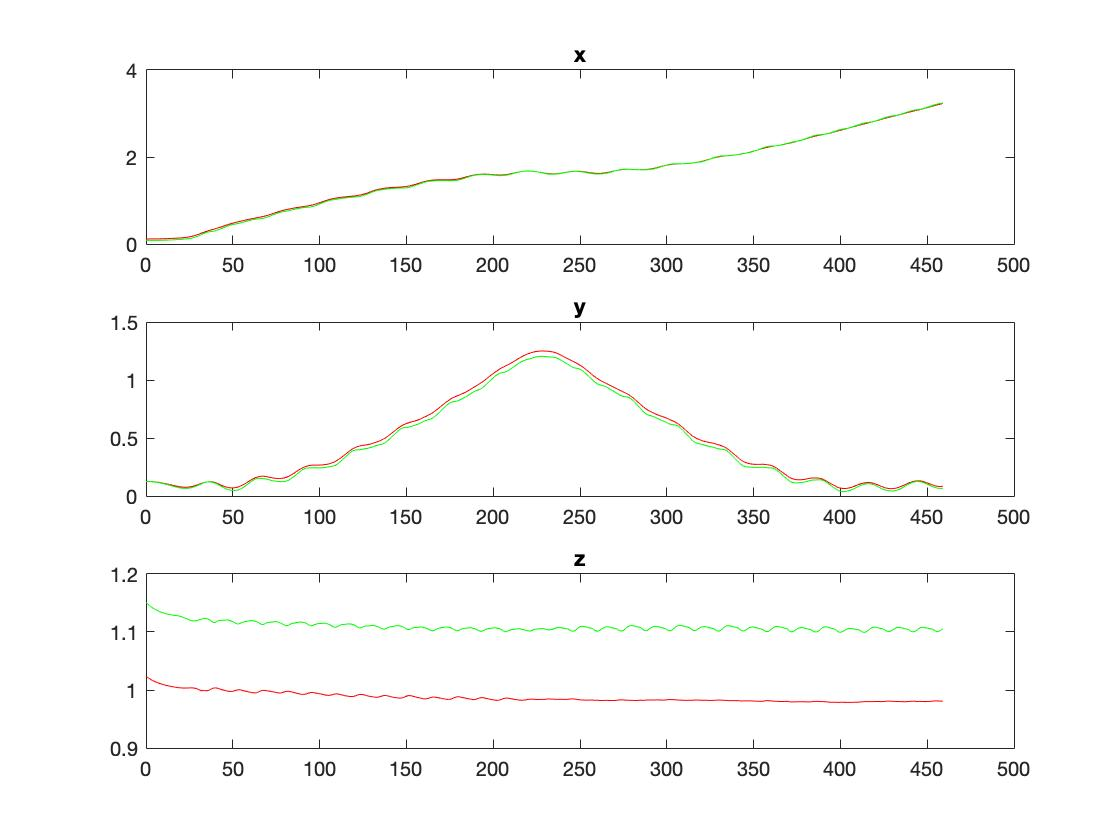
\includegraphics[width=\textwidth]{images/comp_estimated_torso_com.jpg}
    \caption{Comparison of the position of the torso
        estimated
        with the EKF (in red) with respect to the CoM (in green). $x$, $y$, $z$ stands for the position
        of the torso expressed in the reference frame of the
        world. $R$, $P$, $Y$ stands for the rotations roll,
        pitch, yaw around the respective axes of the
        reference frame of the world.}
    \label{fig:comp_estimated_torso_com}
\end{figure}

\begin{figure}
    \centering
    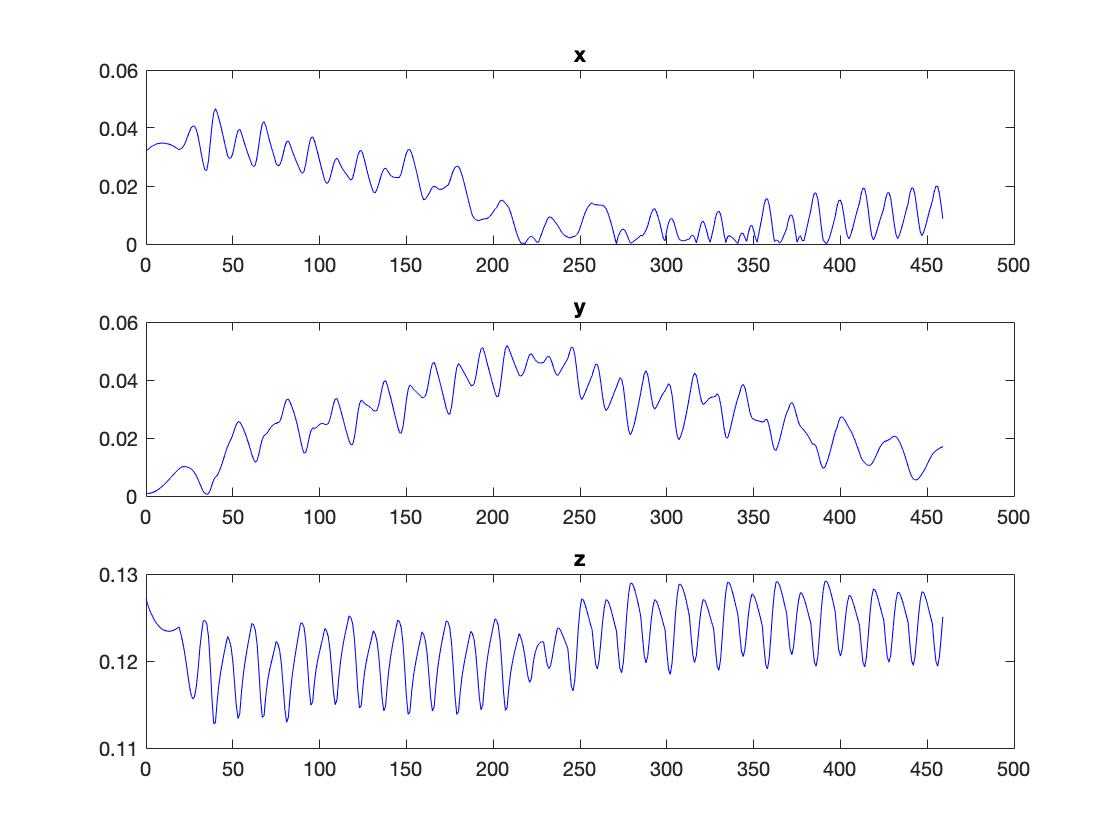
\includegraphics[width=\textwidth]{images/diff_estimated_torso_com.jpg}
    \caption{Difference of the position of the torso
        estimated
        with the EKF (in red) with respect to the CoM (in
        green). $x$, $y$, $z$ stands for the position
        of the torso expressed in the reference frame of the
        world. $R$, $P$, $Y$ stands for the rotations roll,
        pitch, yaw around the respective axes of the
        reference frame of the world.}
    \label{fig:diff_estimated_torso_com}
\end{figure}

\section{Conclusions}
Summary of the project, possible future developments and
conclusions.

%++++++++++++++++++++++++++++++++++++++++
% References section will be created automatically 
% with inclusion of "thebibliography" environment
% as it shown below. See text starting with line
% \begin{thebibliography}{99}
% Note: with this approach it is YOUR responsibility to put them in order
% of appearance.

\bibliography{bibliography} 
\bibliographystyle{ieeetr}

%\begin{thebibliography}{99}

%\bibitem{melissinos}
%A.~C. Melissinos and J. Napolitano, \textit{Experiments in Modern Physics},
%(Academic Press, New York, 2003).

%\bibitem{Cyr}
%N.\ Cyr, M.\ T$\hat{e}$tu, and M.\ Breton,
% "All-optical microwave frequency standard: a proposal,"
%IEEE Trans.\ Instrum.\ Meas.\ \textbf{42}, 640 (1993).

%\bibitem{Wiki} \emph{Expected value},  available at
%\texttt{http://en.wikipedia.org/wiki/Expected\_value}.

%\end{thebibliography}


\end{document}
